% ==========================================================================
% European Journal of Physics 'Paper' (~4000 words) version of qsol_cqed.tex,
% using IOP's current iopjournal.cls template (2024).  On Overleaf: create the
% project from the "IOP Publishing" journal template (it ships iopjournal.cls and
% the orcid icon), replace main.tex with this file, and upload the figures into
% a folder named figures/.  Content is identical to the REVTeX version.
% Generated by scratchpad/make_ejp_iopjournal.py from paper/qsol_cqed.tex.
% Options: \documentclass[anonymous]{iopjournal} strips author details,
% acknowledgments and the data statement for double-anonymous review.
% ==========================================================================
\documentclass{iopjournal}
% graphicx, fancyhdr, xcolor and hyperref are loaded by the class.
\usepackage{amsmath}
\usepackage{amssymb}
\graphicspath{{figures/}{../figures/}}
% running head placeholders (volume/year/article number are set by the journal)
\fancyhead[L]{{\small \sf IOP Publishing}\hspace{5mm} {\it Eur. J. Phys.} {\bf vv} (yyyy) aaaaaa}
\fancyhead[R]{N K Nguyen}

\begin{document}

\articletype{Paper}

\title{Quantum states of light in cavity QED: a computational study of Wigner function dynamics and atom--field entanglement in the Jaynes--Cummings model}

% To add an ORCID iD use \orcid{0000-0000-0000-0000} after the name; it needs the
% "orcid" icon file that ships with the Overleaf IOP template.
\author{Nguyen Khoi Nguyen$^{1,2,*}$}

\affil{$^1$Department of Electrical and Computer Engineering, Boston University, Boston, MA 02215, United States of America}

\affil{$^2$Physics Department, Boston University, Boston, MA 02215, United States of America}

\affil{$^*$Author to whom any correspondence should be addressed.}

\email{nknguyen@bu.edu}  % confirm the address to be published

\keywords{Jaynes--Cummings model, Wigner function, Schr\"{o}dinger cat state, entanglement entropy, decoherence, cavity QED, computational physics education, QuTiP}

\begin{abstract}
The Jaynes--Cummings (JC) model is the standard first encounter with quantized light--matter interaction, yet most courses stop at the collapse and revival of Rabi oscillations and leave three of its most instructive lessons untaught: what the cavity field looks like in phase space while the oscillations are collapsed, how the atom--field entanglement evolves through a collapse--revival cycle, and how quickly cavity loss erases the non-classical features. We present a self-contained computational treatment of these questions for advanced undergraduate and beginning graduate students, in which every figure is generated by a short QuTiP script that the reader can run and modify. Starting from the dipole Hamiltonian we derive the JC model, its dressed states, and the collapse and revival times $t_c = O(1/g)$ and $t_r = 2\pi\sqrt{\bar{n}}/g$, then solve the Lindblad master equation for an initially excited atom and a coherent field with $\bar{n} = 10$. Three results organize the discussion. (i) At half the revival time the field is a Schr\"{o}dinger cat state with Wigner negativity $\delta = 0.85$, purity 0.96 and fidelity 0.78 to a two-component cat, and the atom has disentangled from it (reduced entropy $S \approx 0.14$~bit); during the preceding collapse the atom and field are instead maximally entangled and the reduced field is a two-branch mixture. (ii) Among coherent, thermal, squeezed and Fock initial fields, this half-revival disentanglement occurs only for the coherent field, and a thermal field saturates the reduced entropy at one bit while its logarithmic negativity stays near 0.2, showing why the reduced entropy measures entanglement only for pure global states. (iii) A cavity decay rate of $\kappa/g = 0.02$ removes over 80\% of the Wigner negativity. We close with exercises built on the code and a mapping of the results onto microwave and circuit-QED parameters.
\end{abstract}

\section{Introduction}
\label{sec:intro}

The Jaynes--Cummings (JC) model~\cite{jaynes1963}, a single two-level atom coupled to a single quantized cavity mode, is the simplest fully quantum description of light--matter interaction and the standard first encounter with it in a quantum-optics course. It predicts phenomena with no classical analog: vacuum Rabi splitting, the collapse and revival of Rabi oscillations~\cite{eberly1980}, and the dynamical generation of Schr\"{o}dinger cat states in the cavity field~\cite{brune1996}, all confirmed in microwave cavity QED~\cite{rempe1987, haroche2006} and in circuit QED with superconducting qubits~\cite{blais2021}.

While the JC model appears in every quantum-optics course, most presentations stop at the collapse and revival of the atomic inversion and leave three of its most instructive lessons untaught: what the cavity field looks like in phase space while the oscillations are collapsed, how the atom--field entanglement evolves through a collapse--revival cycle, and how quickly cavity loss erases the non-classical features. The lessons are not new to the research literature. Eberly \textit{et al.}~\cite{eberly1980} explained the collapse and revival, Gea-Banacloche~\cite{gea-banacloche1990, gea-banacloche1991} showed that the atom and field disentangle at half the revival time and leave the field in a Schr\"{o}dinger cat state, and Phoenix and Knight~\cite{phoenix1988, phoenix1991} traced the entanglement entropy through the cycle. They are, however, easy to misread. The cat state and the peak of the entanglement both occur while the inversion is collapsed, and it is tempting to identify one with the other; separating them requires watching the Wigner function, the field purity and the atomic entropy at the same time, which is exactly what a computational treatment makes cheap.

This paper is written for advanced undergraduate and beginning graduate students, and for instructors of quantum-optics or computational-physics courses. It assumes second quantization of a single mode, density matrices and the partial trace, and a first exposure to master equations; Section~\ref{sec:theory} collects the results we need and points to full derivations. Every figure is produced by a short, documented QuTiP~\cite{johansson2012, johansson2013} script that runs in seconds to a minute on a laptop, and the scripts are the intended instrument: the reader is meant to change $\bar{n}$, $\kappa/g$ or the initial field state and watch the figures respond. Section~\ref{sec:teaching} collects exercises built on that premise.

Our contribution relative to textbook treatments~\cite{gerry2004, haroche2006} is threefold. We compute the time-resolved Wigner function of the cavity field and quantify its non-classicality by the negativity volume; we compare the entanglement dynamics across coherent, thermal, squeezed-vacuum and Fock initial fields, using the reduced entropy where the global state is pure and the logarithmic negativity where it is mixed, so that the limits of the entropy as an entanglement measure become visible; and we quantify how cavity dissipation destroys the cat state. The pedagogical core is a three-regime picture: an entangled two-branch mixture during the collapse, a disentangled and nearly pure cat state at half the revival time, and re-entanglement at the revival.

Section~\ref{sec:theory} summarizes the theory, Section~\ref{sec:methods} the computational methods, and Section~\ref{sec:results} the results; Section~\ref{sec:experiment} maps them onto experimental platforms, Section~\ref{sec:teaching} suggests classroom use, and Section~\ref{sec:conclusions} concludes.

\section{Theoretical Framework}
\label{sec:theory}

\subsection{The Jaynes--Cummings model}
\label{sec:jcm}
A single cavity mode is a harmonic oscillator with ladder operators $a$, $a^\dagger$, $[a, a^\dagger] = 1$, and Fock states $|n\rangle$ with $a^\dagger|n\rangle = \sqrt{n+1}\,|n{+}1\rangle$. In the dipole and rotating-wave approximations, a two-level atom with transition frequency $\omega_a$ coupled to the mode of frequency $\omega_c$ is described by the Jaynes--Cummings Hamiltonian~\cite{jaynes1963, gerry2004}
\begin{equation}
H_{\text{JC}} = \hbar\omega_c\, a^\dagger a + \tfrac{1}{2}\hbar\omega_a\sigma_z + \hbar g\left(a^\dagger \sigma^- + a\,\sigma^+\right),
\label{eq:HJC}
\end{equation}
where $\sigma^\pm$ raise and lower the atom, $\sigma_z = |e\rangle\langle e| - |g\rangle\langle g|$, and $g$ is the vacuum Rabi coupling. $H_{\text{JC}}$ conserves the excitation number $a^\dagger a + \sigma^+\sigma^-$, so it decomposes into $2\times 2$ blocks spanned by $\{|e,n\rangle, |g,n{+}1\rangle\}$. With detuning $\Delta = \omega_a - \omega_c$ and $\Omega_0 = 2g$, each block has eigenvalues $E_\pm(n) = \hbar\omega_c(n + \tfrac{1}{2}) \pm \tfrac{1}{2}\hbar\,\Omega_n(\Delta)$ with the $n$-photon Rabi frequency $\Omega_n(\Delta) = \sqrt{\Delta^2 + \Omega_0^2(n+1)}$. Its eigenstates, the dressed states, are equal superpositions of $|e,n\rangle$ and $|g,n{+}1\rangle$ on resonance and approach the bare states in the dispersive limit $|\Delta| \gg \Omega_0\sqrt{n+1}$, where the coupling reduces to ac Stark shifts~\cite{haroche2006}.\label{sec:limits}

\subsection{Collapse and revival}
\label{sec:collapse_revival}
For the atom initially excited and the field in a Fock state $|n\rangle$, on resonance,
\begin{equation}
|\Psi(t)\rangle = \cos\!\left(\tfrac{1}{2}\Omega_n t\right)|e,n\rangle - i\sin\!\left(\tfrac{1}{2}\Omega_n t\right)|g,n{+}1\rangle, \qquad \Omega_n = \Omega_0\sqrt{n+1},
\label{eq:rabi_evolution}
\end{equation}
so the excited-state probability oscillates as $P_e(t) = \cos^2(\tfrac{1}{2}\Omega_n t)$; $n = 0$ is the vacuum Rabi oscillation. For a coherent field $|\alpha\rangle$ with Poissonian statistics $p(n) = e^{-\bar{n}}\bar{n}^n/n!$ and $\bar{n} = |\alpha|^2$, each Fock component evolves independently and
\begin{equation}
P_e(t) = \frac{1}{2} + \frac{1}{2}\sum_{n=0}^{\infty} p(n)\cos\!\left(\Omega_0\sqrt{n+1}\,t\right).
\label{eq:pe_cos_sum}
\end{equation}
The Rabi frequencies of the components spread by $\delta\Omega \approx \Omega_0/2$ across the Poisson width $\sqrt{\bar{n}}$, so the oscillations dephase on the collapse time $t_c \sim 1/g$, independent of $\bar{n}$; linearizing $\sqrt{n+1}$ about $\bar{n}$ gives the envelope $\tfrac{1}{2}\cos(\Omega_0\sqrt{\bar{n}}\,t)\,e^{-g^2t^2/2}$~\cite{eberly1980}. Throughout we use the operational definition $t_c \equiv 1/g$. Because the spectrum is discrete, adjacent components rephase when $(\Omega_0\sqrt{n+2} - \Omega_0\sqrt{n+1})\,t_r = 2\pi$, giving the revival time
\begin{equation}
t_r = \frac{2\pi\sqrt{\bar{n}}}{g},
\label{eq:t_revival}
\end{equation}
a direct signature of field quantization~\cite{eberly1980, haroche2006}. A thermal field, with Bose--Einstein statistics $p(n) = \bar{n}^n/(1+\bar{n})^{n+1}$ and width $\sim\bar{n}$, dephases within a Rabi period and shows no resolved revival; a Fock field never dephases. During the collapse the atom and field become strongly entangled. At half the revival time, $t_r/2 = \pi\sqrt{\bar{n}}/g$, the two branches of the atomic state reconverge, the atom and field approximately \emph{disentangle}, and the field is left in a Schr\"{o}dinger cat state, a superposition of two coherent states with opposite phases~\cite{gea-banacloche1990, gea-banacloche1991, phoenix1991}.

\subsection{Phase space, dissipation, and entanglement measures}
\label{sec:lindblad}
The Wigner function of the reduced field state $\rho_{\text{field}}$~\cite{wigner1932},
\begin{equation}
W(x, p) = \frac{1}{\pi\hbar}\int_{-\infty}^{\infty} \langle x - y | \rho_{\text{field}} | x + y \rangle\, e^{2ipy/\hbar}\, dy,
\label{eq:wigner_def}
\end{equation}
is the Gaussian $\pi^{-1}\exp[-(x - \sqrt{2}\,\text{Re}\,\alpha)^2 - (p - \sqrt{2}\,\text{Im}\,\alpha)^2]$ for a coherent state and takes negative values for Fock and cat states. Negativity is a sufficient but not a necessary witness of non-classicality~\cite{hudson1974}: the squeezed vacuum has a non-negative Gaussian $W$ yet a singular Glauber--Sudarshan $P$ function~\cite{glauber1963, sudarshan1963}. We quantify negativity by the volume~\cite{kenfack2004}
\begin{equation}
\delta = \int \big|W(x,p)\big|\, dx\, dp - 1,
\label{eq:negativity}
\end{equation}
which equals twice the integrated negative part of $W$ because $\int W\,dx\,dp = 1$.

Cavity photon loss at rate $\kappa$ and atomic decay at rate $\gamma$ enter through the Lindblad master equation~\cite{lindblad1976, wiseman2009}
\begin{equation}
\frac{d\rho}{dt} = -\frac{i}{\hbar}[H_{\text{JC}}, \rho] + \kappa\,\mathcal{D}[a]\rho + \gamma\,\mathcal{D}[\sigma^-]\rho, \qquad \mathcal{D}[L]\rho = L\rho L^\dagger - \tfrac{1}{2}\{L^\dagger L, \rho\}.
\label{eq:lindblad}
\end{equation}
The interference fringes of a superposition of two coherent states separated by $\Delta\alpha$ decay at the rate $\kappa|\Delta\alpha|^2/2$~\cite{zurek2003, haroche2006}; for the JC cat, whose components sit at $\pm i\sqrt{\bar{n}}$ (Sec.~\ref{sec:wigner_results}), this is $2\kappa\bar{n}$, far faster than the energy decay rate $\kappa$.

For a pure atom--field state the entanglement is measured by the von Neumann entropy of the reduced atom~\cite{nielsen2000},
\begin{equation}
S(\rho_{\text{atom}}) = -\text{Tr}\big[\rho_{\text{atom}} \log_2 \rho_{\text{atom}}\big],
\label{eq:entropy}
\end{equation}
which ranges from 0 to 1~bit and is complemented by the field purity $\mathcal{P} = \text{Tr}[\rho_{\text{field}}^2]$. If the global state is mixed, as for a thermal field or under dissipation, $S(\rho_{\text{atom}})$ counts classical correlations as well and can reach 1~bit for a weakly entangled state; we then use the logarithmic negativity~\cite{vidal2002, plenio2005}
\begin{equation}
E_{\mathcal{N}} = \log_2 \big\| \rho^{T_{\text{atom}}} \big\|_1,
\label{eq:logneg}
\end{equation}
an entanglement monotone that vanishes for separable states and equals 1 for a maximally entangled pair. Phoenix and Knight~\cite{phoenix1988, phoenix1991} first traced $S$ through the collapse--revival cycle; Sec.~\ref{sec:results} verifies that picture computationally.


\section{Computational Methods}
\label{sec:methods}

All simulations are performed using QuTiP (Quantum Toolbox in Python, version~5.2)~\cite{johansson2012, johansson2013}, an open-source framework for simulating open and closed quantum systems. The cavity field is represented in a truncated Fock basis $\{|0\rangle, |1\rangle, \ldots, |N_{\text{cav}}-1\rangle\}$, and the joint atom--field Hilbert space has dimension $2N_{\text{cav}}$.

\textit{Fock space truncation.} The truncation is chosen per initial state. For the coherent and Fock states with $\bar{n} = 10$ we use $N_{\text{cav}} = 35$--$50$: the Poisson weight beyond $n = 35$ is below $10^{-9}$, and every quantity reported at $t_r/2$ (entropy, purity, $\delta$) agrees to four digits between $N_{\text{cav}} = 35$, 50, and 70. Thermal and squeezed-vacuum fields have much heavier photon-number tails (geometric, and $\propto \tanh^{2m}r/\sqrt{m}$ for $n = 2m$, respectively): at $N_{\text{cav}} = 50$ the truncated states would have $\langle n\rangle = 9.57$ and $9.15$ instead of 10, so for these we use $N_{\text{cav}} = 150$, which reproduces $\langle n\rangle = 10$ to four digits and leaves a truncated weight below $10^{-6}$. For the $\bar{n}$ scan we use $N_{\text{cav}} = 3\bar{n} + 20$. Trace normalization alone is not used as a convergence criterion.

\textit{Time evolution.} All propagation uses QuTiP's \texttt{mesolve} (version 5.2.3) with its default adaptive-step Adams--Moulton multistep integrator (\texttt{method='adams'}, absolute and relative tolerances $10^{-8}$ and $10^{-6}$). Pure initial states without dissipation are propagated as state vectors; the thermal initial field and all dissipative runs [Eq.~(\ref{eq:lindblad})] propagate the full density matrix.

\textit{Wigner functions.} At each snapshot time, we obtain the reduced field state $\rho_{\text{field}}(t) = \text{Tr}_{\text{atom}}[\rho(t)]$ via partial trace, then compute $W(x,p)$ on a $200 \times 200$ grid over $[-7, 7]^2$ (spacing 0.07, i.e.\ ten points per interference fringe of spacing $\pi/\sqrt{2\bar{n}} \approx 0.70$) using QuTiP's \texttt{wigner} function~\cite{johansson2012} in the convention $a = (x + ip)/\sqrt{2}$, for which $\int W\,dx\,dp = 1$ (verified to $10^{-4}$ on the grid). The negativity $\delta$ of Eq.~(\ref{eq:negativity}) is evaluated on the same grid.

\textit{Entanglement and cat-state measures.} The von Neumann entropy $S(\rho_{\text{atom}})$ is computed at each time step from the eigenvalues of the $2 \times 2$ reduced atomic density matrix, the field purity $\mathcal{P}(t) = \text{Tr}[\rho_{\text{field}}^2]$ directly, and the logarithmic negativity of Eq.~(\ref{eq:logneg}) from the trace norm of the partially transposed joint state. The cat-state fidelity is $F_{\text{cat}} = \max\,\langle \text{cat}|\rho_{\text{field}}|\text{cat}\rangle$ over normalized states $|\text{cat}\rangle \propto |\beta\rangle + e^{i\theta}|{-\beta}\rangle$, with $\beta$ scanned in a neighborhood of $i\sqrt{\bar{n}}$ and $\theta \in [0, 2\pi)$.

\textit{Parameters.} We work in dimensionless units with $g = 1$. The characteristic timescales are the collapse time $t_c \equiv 1/g$ and the revival time $t_r = 2\pi\sqrt{\bar{n}}/g$. Table~\ref{tab:params} summarizes the simulation parameters.

\begin{table}
\centering
\caption{Simulation parameters. All quantities in units where $g = 1$ and $\hbar = 1$.}
\begin{tabular}{lcccc}
\hline
Simulation & $\bar{n}$ & $N_{\text{cav}}$ & $\kappa/g$ & $\gamma/g$ \\
\hline
Wigner evolution & 10 & 35 & 0 & 0 \\
Entanglement (coherent, Fock) & 10 & 50 & 0 & 0 \\
Entanglement (thermal, squeezed) & 10 & 150 & 0 & 0 \\
$\bar{n}$ scaling & 1--36 & $3\bar{n}+20$ & 0 & 0 \\
Dissipative dynamics & 10 & 35--50 & 0--0.2 & 0 \\
\hline
\end{tabular}
\label{tab:params}
\end{table}

All simulation code is available as Python scripts at \url{https://github.com/alanknguyen/QSOL_CQED}.


\section{Results and Discussion}
\label{sec:results}

\subsection{Wigner function evolution and cat-state formation}
\label{sec:wigner_results}

We first consider unitary JC dynamics with the atom initially excited and the field in a coherent state $|\alpha\rangle$ with $\bar{n} = |\alpha|^2 = 10$. Figure~\ref{fig:inversion_snapshots} shows the atomic inversion $\langle\sigma_z(t)\rangle$, exhibiting the collapse-revival structure: rapid Rabi oscillations that dephase by $t \approx 2/g$, a quiescent interval, and a revival centered at $t_r \approx 2\pi\sqrt{10}/g \approx 19.9/g$.

\begin{figure}
\centering
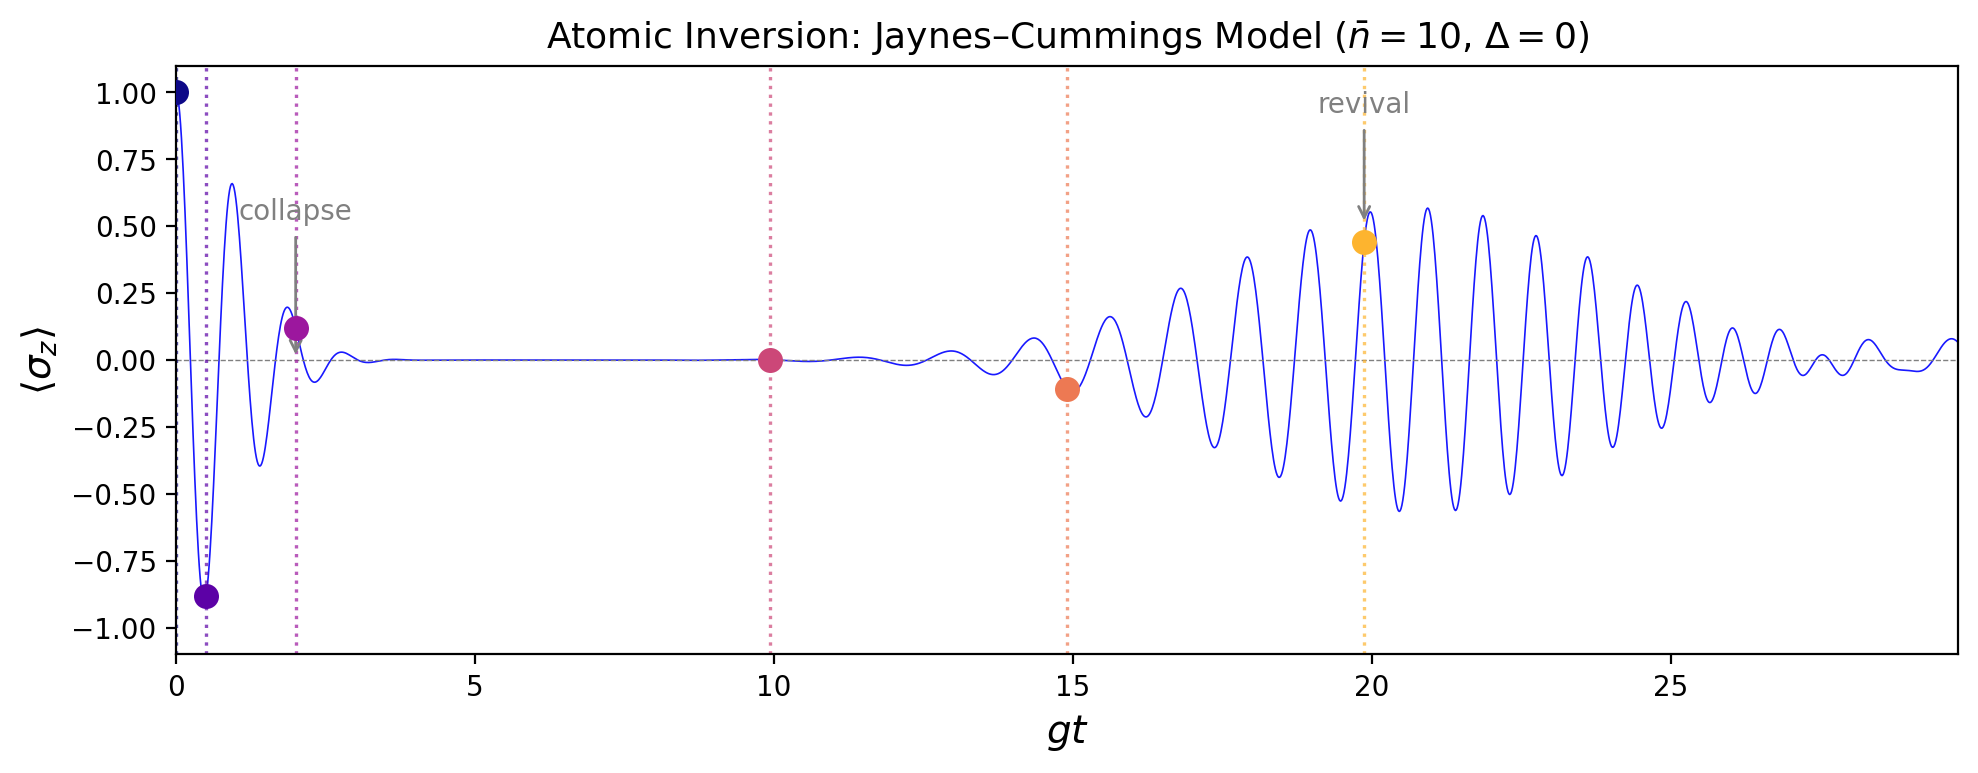
\includegraphics[width=\textwidth]{fig_inversion_snapshots.png}
\caption{Atomic inversion $\langle\sigma_z(t)\rangle$ for a two-level atom interacting with a coherent-state field ($\bar{n} = 10$) in the resonant Jaynes--Cummings model. Colored markers indicate the six snapshot times used for the Wigner function evolution in Fig.~\ref{fig:wigner_evolution}. The collapse of oscillations near $t \approx 2/g$ and the first revival at $t_r \approx 19.9/g$ are clearly visible.}
\label{fig:inversion_snapshots}
\end{figure}

\begin{figure}
\centering

\includegraphics[width=\textwidth]{fig_wigner_evolution.png}
\caption{Wigner function $W(x,p)$ of the reduced cavity field state at six characteristic times during Jaynes--Cummings evolution ($\bar{n} = 10$, $\Delta = 0$). At $t = 0$, the field is a coherent-state Gaussian. By $t = 2\,t_c$ (collapse onset), the distribution begins to spread. At $t = t_r/2$, a Schr\"{o}dinger cat state has formed: two distinct lobes at $p \approx \pm\sqrt{2\bar{n}}$ connected by interference fringes with strong Wigner negativity ($\delta = 0.85$); at this time the atom and field are approximately disentangled (Sec.~\ref{sec:entropy_results}). By $t = t_r$, the field partially re-localizes at revival ($\delta = 0.31$).}
\label{fig:wigner_evolution}
\end{figure}

The central computational result of this section is shown in Fig.~\ref{fig:wigner_evolution}, which displays the Wigner function of the reduced cavity field at six characteristic times. At $t = 0$, the Wigner function is a Gaussian displaced to $x \approx 4.5$, consistent with the initial coherent state. As the system evolves through the collapse region ($t \approx 2/g$), the distribution spreads along the circle $x^2 + p^2 = 2\bar{n}$ in phase space. At the midpoint of the collapse--revival cycle ($t = t_r/2$), the Wigner function develops two well-separated lobes connected by interference fringes with alternating positive and negative values, the signature of a Schr\"{o}dinger cat state, $|\Psi_{\text{cat}}\rangle \approx \mathcal{N}(|\beta\rangle + e^{i\theta}|{-\beta}\rangle)$ with $\beta \approx i\sqrt{\bar{n}}$: the two components sit on the $p$ axis, rotated by $\pm\pi/2$ from the initial coherent amplitude.

Figure~\ref{fig:cat_detail} provides a detailed view of this cat state. The cross-section $W(x, p = 0)$ shows deep negative excursions reaching $W \approx -0.25$, with Wigner negativity volume $\delta = 0.85$ (compared to $\delta = 0$ at $t = 0$). The best-fitting two-component cat has fidelity $F_{\text{cat}} = 0.78$ with the reduced field state, whose purity is $\mathcal{P} = 0.96$: the field is a nearly pure cat state rather than one branch of an entangled atom--field pair (Sec.~\ref{sec:entropy_results}). The relative phase of the fit is $\theta \approx 1.2\pi$ and the photon-number parity is $\langle(-1)^{\hat{n}}\rangle = -0.64$, so the JC cat is closer to an odd than to an even cat, and its photon-number distribution displays the corresponding odd-$n$ comb; its fidelity with the even cat $|\alpha\rangle + |{-\alpha}\rangle$ on the real axis is essentially zero. The interference fringes have characteristic spacing $\Delta x \approx \pi/\sqrt{2\bar{n}} \approx 0.7$, set by the separation of the two coherent components. These fringes are the phase-space manifestation of quantum interference between macroscopically distinguishable field states and serve as a definitive marker of non-classicality.

\begin{figure}
\centering

\includegraphics[width=\textwidth]{fig_cat_state_detail.png}
\caption{Detailed view of the Schr\"{o}dinger cat state formed at $t = t_r/2$. Left: Wigner function contour plot showing two coherent-state lobes and interference fringes. Right: cross-section $W(x, p=0)$ with negative regions (shaded red) reaching $W \approx -0.25$; the fringe spacing is $\pi/\sqrt{2\bar{n}} \approx 0.70$. The negativity ($\delta = 0.85$) confirms the non-classical character of this dynamically generated state, whose fidelity with the best-fitting two-component cat is 0.78.}
\label{fig:cat_detail}
\end{figure}

As the system approaches the revival time, the two lobes merge and the Wigner function partially re-localizes, though with residual non-classical features ($\delta = 0.31$ at $t = t_r$). The revival is not exact: higher-order terms in the photon-number distribution prevent perfect recurrence. Negative $W$ is the phase-space face of the non-classicality that photon counting detects as sub-Poissonian statistics or antibunching~\cite{kimble1977}; the Glauber--Sudarshan $P$ function remains the definitive criterion, and the everywhere-positive Husimi $Q$ function is correspondingly less sensitive.


\subsection{Atom--field entanglement dynamics}
\label{sec:entropy_results}

We now quantify atom--field entanglement, comparing four initial field states with the same mean photon number $\bar{n} = 10$: coherent, thermal, squeezed vacuum, and Fock. For the three pure initial fields the global state remains pure and $S(\rho_{\text{atom}})$ is the entanglement entropy; for the thermal field we report both $S$ and the logarithmic negativity $E_{\mathcal{N}}$ of Eq.~(\ref{eq:logneg}).

Figure~\ref{fig:entanglement_comparison} shows the inversion, entropy, and negativity for all four cases. The principal observations are as follows.

\begin{figure}
\centering

\includegraphics[width=0.85\textwidth]{fig_entanglement_comparison.png}
\caption{Comparison of Jaynes--Cummings dynamics for four initial field states with $\bar{n} = 10$. (a) Atomic inversion $\langle\sigma_z\rangle$ for the coherent (blue), thermal (red), and squeezed-vacuum (green) fields. (b) Fock state $|10\rangle$ over a short window: the inversion oscillates with period $\pi/(g\sqrt{11})$ and the entropy (plotted as $2S - 1$) with half that period. (c) Reduced-atom entropy $S(\rho_{\text{atom}})$ (solid) and logarithmic negativity $E_{\mathcal{N}}$ (dashed). The coherent state collapses to $S \approx 1$~bit and disentangles at $t_r/2$ (dotted line); the thermal state saturates at $S = 1$~bit but has $E_{\mathcal{N}} \approx 0.2$ because its global state is mixed; the squeezed vacuum shows only partial dips. The dashed purple line marks the revival time $t_r$.}
\label{fig:entanglement_comparison}
\end{figure}

\textit{Coherent state.} The entropy rises from $S = 0$ to $\approx 1$~bit within $t \approx 2/g$, as the Rabi oscillations collapse. It then decreases steadily and reaches a minimum $S \approx 0.14$~bit ($E_{\mathcal{N}} = 0.36$) at $t = t_r/2 \approx 9.9/g$, in the middle of the quiescent interval. This is the half-revival disentanglement predicted by Gea-Banacloche~\cite{gea-banacloche1990}: the atom returns close to a pure state while the field is in the cat state of Fig.~\ref{fig:cat_detail}. Toward the revival the entanglement grows again; at $t_r$ the entropy is $S \approx 0.79$~bit and oscillates between about 0.5 and 1 at the Rabi frequency. The cat state and the minimum of entanglement therefore coincide: the field is a nearly pure superposition, not one branch of an entangled pair.

\textit{Thermal state.} The reduced entropy rises to $S = 1$~bit within $t \sim 1/g$ and stays within a few percent of the maximum thereafter, with no dip at $t_r/2$. This does not indicate maximal entanglement: the global state is mixed, and the logarithmic negativity remains small, $E_{\mathcal{N}} \approx 0.23$ on average (maximum 0.33). Most of the reduced-atom entropy is classical correlation inherited from the broad Bose--Einstein photon distribution, whose spread of Rabi frequencies ($\sigma_n \sim \bar{n}$) dephases the oscillations within a Rabi period and leaves no resolved revival in the simulated window.

\textit{Squeezed vacuum.} The dynamics are intermediate: a rapid rise to $S \approx 1$~bit followed by quasi-periodic partial dips (to $S \approx 0.7$--$0.8$), but no clean half-revival disentanglement. The super-Poissonian photon statistics of the squeezed vacuum (only even $n$ populated, variance $2\bar{n}(\bar{n}+1)$) spread the Rabi frequencies over a much wider range than the Poisson distribution.

\textit{Fock state.} With a definite photon number there is a single Rabi frequency, $\Omega_{10} = 2g\sqrt{11}$ [Eq.~(\ref{eq:rabi_evolution})]. The inversion oscillates with period $\pi/(g\sqrt{11}) \approx 0.95/g$, and the entropy, which depends on the populations only through the binary entropy $h(P_e)$ with $h(p) = h(1-p)$, oscillates between 0 and 1~bit with half that period, $\pi/(2g\sqrt{11}) \approx 0.47/g$ [Fig.~\ref{fig:entanglement_comparison}(b)]. No collapse or revival occurs because there is no dephasing.

Figure~\ref{fig:coherent_detail} shows the coherent-state case in greater detail, plotting inversion, entropy, and field purity $\mathcal{P}(t)$ together. During the collapse the field purity drops to $\mathcal{P} \approx 0.5$: the reduced field is then an incoherent \emph{mixture} of two nearly orthogonal branches, each correlated with a different atomic state (a coherent superposition of the two branches would have $\mathcal{P} = 1$). As the atomic branches reconverge, the purity climbs to $\mathcal{P} = 0.96$ at $t_r/2$, where the field is the nearly pure cat, and falls again toward the revival ($\mathcal{P} = 0.64$ at $t_r$). The three observables thus tell a single story: entanglement during the collapse turns the reduced field into a two-branch mixture, and disentanglement at $t_r/2$ restores the field's coherence in the form of a cat state.

\begin{figure}
\centering

\includegraphics[width=0.85\textwidth]{fig_coherent_entropy_purity.png}
\caption{Detailed coherent-state dynamics ($\bar{n} = 10$). Top: atomic inversion. Middle: entanglement entropy $S(\rho_{\text{atom}})$, peaking near 1~bit during the collapse and reaching its minimum ($\approx 0.14$~bit) at $t_r/2$, where the atom and field disentangle and the field is the cat state of Fig.~\ref{fig:cat_detail}. Bottom: field purity $\mathcal{P} = \text{Tr}[\rho_{\text{field}}^2]$, dropping to $\approx 0.5$ during the collapse (a two-branch mixture, the field being entangled with the atom) and rising to 0.96 at $t_r/2$ (nearly pure cat). Dotted and dashed lines mark $t_r/2$ and $t_r$.}
\label{fig:coherent_detail}
\end{figure}

Figure~\ref{fig:entropy_nbar} shows how these dynamics depend on $\bar{n}$. For $\bar{n} = 1$ the entropy oscillates quasi-periodically without a clean collapse. As $\bar{n}$ increases, the collapse still occurs at $t \sim 1/g$, but the half-revival minimum at $\pi\sqrt{\bar{n}}/g$ moves out and deepens ($S_{\min} \approx 0.16$, 0.11, 0.07, and 0.05~bit for $\bar{n} = 9$, 16, 25, and 36), and the entangled plateau around the revival broadens. For $\bar{n} \gtrsim 9$ the disentanglement and the subsequent re-entanglement are cleanly resolved, consistent with the large-$\bar{n}$ analysis of Gea-Banacloche~\cite{gea-banacloche1991}.

\begin{figure}
\centering

\includegraphics[width=\textwidth]{fig_entropy_nbar_scaling.png}
\caption{Entanglement entropy $S(\rho_{\text{atom}})$ for coherent-state fields with $\bar{n} = 1,\, 4,\, 9,\, 16,\, 25,\, 36$. As $\bar{n}$ increases, the collapse time remains $\sim 1/g$ while the half-revival time $\pi\sqrt{\bar{n}}/g$ (dotted) and the revival time $t_r = 2\pi\sqrt{\bar{n}}/g$ (dashed) grow as $\sqrt{\bar{n}}$. The entropy minimum at $t_r/2$ (atom--field disentanglement) deepens with $\bar{n}$ and is cleanly resolved for $\bar{n} \gtrsim 9$.}
\label{fig:entropy_nbar}
\end{figure}


\subsection{Decoherence of non-classical features}
\label{sec:decoherence}

We now include cavity photon loss ($\kappa > 0$) via Eq.~(\ref{eq:lindblad}) and study its effect on the Wigner function and entanglement.

Figure~\ref{fig:wigner_decoherence} shows the Wigner function at the cat-state time $t = t_r/2$ for $\kappa/g = 0,\, 0.02,\, 0.05,\, 0.10$. The interference fringes are progressively destroyed: at $\kappa/g = 0.02$, the Wigner negativity drops from $\delta = 0.85$ to $\delta = 0.14$; at $\kappa/g = 0.10$, the negativity is effectively zero ($\delta = 0.002$). Table~\ref{tab:decoherence} summarizes these results; the values are converged to three digits between $N_{\text{cav}} = 35$ and 50.

\begin{figure}
\centering

\includegraphics[width=\textwidth]{fig_wigner_decoherence.png}
\caption{Decoherence of the Schr\"{o}dinger cat state. Wigner function at $t = t_r/2$ for increasing cavity decay rates $\kappa/g = 0,\, 0.02,\, 0.05,\, 0.10$ (left to right). The interference fringes are progressively destroyed; quantitative values of the Wigner negativity $\delta$ are given in Table~\ref{tab:decoherence}.}
\label{fig:wigner_decoherence}
\end{figure}

\begin{table}
\centering
\caption{Wigner negativity $\delta$ and field purity $\mathcal{P}$ at $t = t_r/2$ for varying cavity decay rate, with $\bar{n} = 10$.}
\begin{tabular}{cccc}
\hline
$\kappa/g$ & Wigner negativity $\delta$ & Field purity $\mathcal{P}$ & Cat state visible? \\
\hline
0.00 & 0.851 & 0.960 & Yes \\
0.02 & 0.143 & 0.460 & Marginal \\
0.05 & 0.022 & 0.418 & No \\
0.10 & 0.002 & 0.386 & No \\
\hline
\end{tabular}
\label{tab:decoherence}
\end{table}

This extreme sensitivity is expected: the fringe decoherence rate is $2\kappa\bar{n}$ (Sec.~\ref{sec:lindblad}). For $\bar{n} = 10$, even $\kappa/g = 0.02$ gives a fringe-decoherence time $1/(2\kappa\bar{n}) = 2.5/g$, a quarter of the cat-formation time $t_r/2 \approx 10/g$, which suffices to wash out most of the interference while the two Gaussian lobes, which decay only at the rate $\kappa$, persist.

Figure~\ref{fig:dissipative_entropy} shows the inversion, the reduced entropy, and the logarithmic negativity under dissipation. Three effects are visible. (i) The Rabi revival is damped and the inversion relaxes toward $\langle\sigma_z\rangle \to -1$ as photons leak out; for $\kappa/g = 0.2$ the atom is essentially in its ground state by $gt \approx 30$. (ii) The reduced entropy no longer measures entanglement: for $\kappa/g \geq 0.05$ it saturates near 1~bit at late times while the negativity decays toward zero ($E_{\mathcal{N}} = 0.14$, 0.02, and 0.00 at $gt = 30$ for $\kappa/g = 0.05$, 0.10, and 0.20). (iii) The atom--field entanglement at $t_r/2$ is comparatively robust: $E_{\mathcal{N}}(t_r/2) \approx 0.35$ for all $\kappa/g \leq 0.1$, close to the unitary value 0.36, even though the entropy minimum is progressively filled in [$S(t_r/2) = 0.14$, 0.16, 0.27, and 0.49 for $\kappa/g = 0$, 0.01, 0.05, and 0.10] and the cat fringes of Table~\ref{tab:decoherence} are already gone at $\kappa/g = 0.05$. Cavity loss thus destroys the internal coherence of the field cat long before it changes the (small) residual entanglement between atom and field.

\begin{figure}
\centering

\includegraphics[width=0.85\textwidth]{fig_dissipative_entanglement.png}
\caption{Effect of cavity decay on JC dynamics ($\bar{n} = 10$). Top: atomic inversion for $\kappa/g = 0$--$0.20$. Middle: reduced-atom entropy, which for $\kappa > 0$ measures total (classical plus quantum) correlations. Bottom: logarithmic negativity $E_{\mathcal{N}}$, a proper entanglement monotone for the mixed states produced by dissipation. Increasing $\kappa$ damps the revival, drives the atom toward its ground state, and suppresses the late-time negativity even where the reduced entropy stays near 1~bit. Dotted and dashed lines mark $t_r/2$ and $t_r$.}
\label{fig:dissipative_entropy}
\end{figure}

These results demonstrate the challenge of maintaining quantum coherence. By the operational criterion $\delta > 0.05$ at $t_r/2$, cat-state formation with $\bar{n} = 10$ requires $\kappa/g \lesssim 0.03$, i.e.\ $g/\kappa \gtrsim 30$; the threshold depends on $\bar{n}$, on the observation time, and on the chosen figure of merit (a full map of $\delta$ and $F_{\text{cat}}$ over the $(\bar{n}, \kappa/g)$ plane is provided with the code). This condition is routinely achieved in microwave cavity QED~\cite{haroche2006} and circuit QED~\cite{blais2021}, but remains an engineering challenge in optical cavities.


\section{Connection to Experiment}
\label{sec:experiment}

Collapse and revival were first observed with Rydberg atoms crossing a superconducting microwave cavity~\cite{rempe1987}; the same platform later generated and detected cat states~\cite{brune1996, haroche2006}, trapped ions reproduced the full sequence with a vibrational mode playing the role of the field~\cite{meekhof1996}, and circuit QED now reaches $g/\kappa \sim 100$--$300$ with superconducting qubits~\cite{blais2021}, where cat states serve as error-corrected qubits~\cite{ofek2016}. Our dimensionless results map onto any platform by inserting the physical value of $g$. For microwave cavity QED ($g/2\pi \sim 50$~kHz, $\kappa/2\pi \sim 1$~Hz) the revival time for $\bar{n} = 10$ is $t_r = 2\pi\sqrt{10}/g \approx 60~\mu$s against a cavity lifetime $1/\kappa \approx 0.16$~s; for circuit QED ($g/2\pi \sim 100$--$300$~MHz, $\kappa/2\pi \sim 1$~MHz) it is $10$--$30$~ns against $160$~ns. The cat fringes, which decay at $2\kappa\bar{n}$, survive only where $\kappa/g \lesssim 0.01$--$0.03$, the threshold of Sec.~\ref{sec:decoherence}; this is met in both regimes but not in typical optical cavities.


\section{Using this material in teaching}
\label{sec:teaching}

This study grew out of a term project in a graduate course on quantum optics at Boston University (EC~585/777) and is organized so that it can be reused in that role.

\textit{Where it fits.} The natural place is immediately after the JC model and the collapse-revival phenomenon have been introduced, in a quantum-optics or cavity-QED course at advanced-undergraduate or first-year-graduate level, or as a case study in a computational-physics module. Prerequisites are second quantization of a single mode, density matrices and the partial trace, and a first exposure to the Lindblad equation; Section~\ref{sec:theory} supplies the rest. Three lectures cover the content: (a) collapse and revival as dephasing and rephasing of a discrete spectrum, using Figs.~\ref{fig:inversion_snapshots} and \ref{fig:entropy_nbar}; (b) the field in phase space, the cat state and its decoherence, using Figs.~\ref{fig:wigner_evolution}, \ref{fig:cat_detail} and \ref{fig:wigner_decoherence} and Table~\ref{tab:decoherence}; (c) entanglement measures and their limits, using Figs.~\ref{fig:entanglement_comparison}, \ref{fig:coherent_detail} and \ref{fig:dissipative_entropy}.

\textit{Misconceptions the figures are designed to confront.} Four statements are tempting and wrong, and each is refuted by a figure the student can regenerate. First, that the cat state forms when the atom and field are maximally entangled: Fig.~\ref{fig:coherent_detail} shows the entropy at its minimum, not its maximum, when the cat appears. Second, that a field purity of one half signals a superposition of two states: it signals a mixture, and the coherent superposition arrives only when the purity returns to 0.96 at $t_r/2$. Third, that a reduced entropy of one bit means maximal entanglement: for the thermal field of Fig.~\ref{fig:entanglement_comparison} the logarithmic negativity is only about 0.2, because the global state is mixed. Fourth, that a non-negative Wigner function implies a classical state: the squeezed vacuum has $\delta = 0$ and is nonetheless non-classical (Sec.~\ref{sec:lindblad}).

\textit{Exercises.} All of the following run in seconds to a minute on a laptop with the scripts in the repository.
\begin{enumerate}
\item Change $\bar{n}$ in the Wigner-evolution script to 4, 16 and 25 and verify from the inversion that $t_r$ scales as $\sqrt{\bar{n}}$ while the collapse is complete by $t \approx 2/g$ regardless.
\item Derive the entropy period $\pi/(2g\sqrt{n+1})$ of the Fock state from Eq.~(\ref{eq:rabi_evolution}) and the symmetry $h(p) = h(1-p)$ of the binary entropy, then confirm it against panel (b) of Fig.~\ref{fig:entanglement_comparison}.
\item Reproduce Table~\ref{tab:decoherence} and extend it to $\kappa/g = 0.01$ and $0.03$; locate the decay rate at which $\delta$ falls below 0.05, and compare with the naive estimate obtained by equating the fringe-decoherence time $1/(2\kappa\bar{n})$ to the formation time $t_r/2$. Explain why the estimate is too conservative.
\item Using the closed form $P(n,t) = p(n)\cos^2(g\sqrt{n+1}\,t) + p(n-1)\sin^2(g\sqrt{n}\,t)$ for the photon-number distribution, show that $P(n, t_r/2)$ alternates with the parity of $n$, and compare the predicted parity $\langle(-1)^{\hat{n}}\rangle$ with the numerical value $-0.64$ quoted in Sec.~\ref{sec:wigner_results}.
\item Repeat the thermal-field simulation with $N_{\text{cav}} = 50$ instead of 150 and explain, from the initial $\langle n\rangle$, why the truncation must be chosen per initial state. This is the convergence check that separates a simulation from a picture.
\item (Advanced) Add a detuning $\Delta \neq 0$ to the Hamiltonian and investigate how the half-revival cat fidelity and the entropy minimum change; relate the result to the dispersive limit of Sec.~\ref{sec:limits}.
\end{enumerate}

\textit{Assessment.} A suitable project is to produce the three-observable portrait of Fig.~\ref{fig:coherent_detail} for a different initial state, for example a displaced Fock state or an initial atomic superposition, and to explain in one page where the cat forms, when the atom and field disentangle, and what the logarithmic negativity adds to the reduced entropy.


\section{Conclusions}
\label{sec:conclusions}

We have presented a computational treatment of the Jaynes--Cummings model intended for teaching, in which the collapse and revival of Rabi oscillations, the phase-space dynamics of the cavity field, and the atom--field entanglement are followed together from reproducible code. Three lessons emerge. First, the Schr\"{o}dinger cat state that forms at half the revival time, with Wigner negativity $\delta = 0.85$, purity 0.96 and cat fidelity 0.78, coincides with a \emph{minimum} of the atom--field entanglement ($S \approx 0.14$~bit): it is a nearly pure state of the field alone, whereas during the preceding collapse the atom and field are maximally entangled and the reduced field is a two-branch mixture. Second, this half-revival disentanglement~\cite{gea-banacloche1990, phoenix1991} is unique to the coherent field, and for a thermal field a reduced entropy of one bit conceals a logarithmic negativity of only about 0.2: once the global state is mixed, the reduced entropy is not an entanglement measure. Third, cavity decay as weak as $\kappa/g = 0.02$ removes over 80\% of the Wigner negativity while leaving the residual atom--field negativity at $t_r/2$ nearly unchanged, separating the loss of the field's internal coherence from the loss of entanglement.

The physics is classical work; what the computational route adds is that the three observables can be placed side by side at negligible cost, so that each misconception listed in Sec.~\ref{sec:teaching} becomes a figure a student can regenerate and then break by changing a parameter.


\ack{The author thanks Prof.\ Luca Dal Negro for guidance and feedback during the preparation of this work (EC 585 and EC 777, Boston University).}

% \funding{This work received no external funding.}
% \roles{N K N carried out all the work reported.}

\data{The simulation code that generates every figure in this article, together with the raw sweep data, is openly available at \url{https://github.com/alanknguyen/QSOL_CQED}. All results were obtained with QuTiP 5.2.3.}

% \suppdata{...}

% thebibliography prints the "References" heading itself in this (article-based) class
\begin{thebibliography}{99}
\bibitem{gerry2004} Gerry C C and Knight P L 2004 {\it Introductory Quantum Optics} (Cambridge: Cambridge University Press)
\bibitem{jaynes1963} Jaynes E T and Cummings F W 1963 {\it Proc. IEEE} {\bf 51} 89
\bibitem{eberly1980} Eberly J H, Narozhny N B and Sanchez-Mondragon J J 1980 {\it Phys. Rev. Lett.} {\bf 44} 1323
\bibitem{brune1996} Brune M, Hagley E, Dreyer J, Ma\^{\i}tre X, Maali A, Wunderlich C, Raimond J M and Haroche S 1996 {\it Phys. Rev. Lett.} {\bf 77} 4887
\bibitem{rempe1987} Rempe G, Walther H and Klein N 1987 {\it Phys. Rev. Lett.} {\bf 58} 353
\bibitem{haroche2006} Haroche S and Raimond J-M 2006 {\it Exploring the Quantum: Atoms, Cavities, and Photons} (Oxford: Oxford University Press)
\bibitem{blais2021} Blais A, Grimsmo A L, Girvin S M and Wallraff A 2021 {\it Rev. Mod. Phys.} {\bf 93} 025005
\bibitem{glauber1963} Glauber R J 1963 {\it Phys. Rev.} {\bf 131} 2766
\bibitem{sudarshan1963} Sudarshan E C G 1963 {\it Phys. Rev. Lett.} {\bf 10} 277
\bibitem{wigner1932} Wigner E 1932 {\it Phys. Rev.} {\bf 40} 749
\bibitem{hudson1974} Hudson R L 1974 {\it Rep. Math. Phys.} {\bf 6} 249
\bibitem{kenfack2004} Kenfack A and \.{Z}yczkowski K 2004 {\it J. Opt. B: Quantum Semiclass. Opt.} {\bf 6} 396
\bibitem{lindblad1976} Lindblad G 1976 {\it Commun. Math. Phys.} {\bf 48} 119
\bibitem{wiseman2009} Wiseman H M and Milburn G J 2009 {\it Quantum Measurement and Control} (Cambridge: Cambridge University Press)
\bibitem{zurek2003} Zurek W H 2003 {\it Rev. Mod. Phys.} {\bf 75} 715
\bibitem{nielsen2000} Nielsen M A and Chuang I L 2000 {\it Quantum Computation and Quantum Information} (Cambridge: Cambridge University Press)
\bibitem{phoenix1988} Phoenix S J D and Knight P L 1988 {\it Ann. Phys. (N.Y.)} {\bf 186} 381
\bibitem{johansson2012} Johansson J R, Nation P D and Nori F 2012 {\it Comput. Phys. Commun.} {\bf 183} 1760
\bibitem{johansson2013} Johansson J R, Nation P D and Nori F 2013 {\it Comput. Phys. Commun.} {\bf 184} 1234
\bibitem{gea-banacloche1990} Gea-Banacloche J 1990 {\it Phys. Rev. Lett.} {\bf 65} 3385
\bibitem{gea-banacloche1991} Gea-Banacloche J 1991 {\it Phys. Rev.} A {\bf 44} 5913
\bibitem{phoenix1991} Phoenix S J D and Knight P L 1991 {\it Phys. Rev.} A {\bf 44} 6023
\bibitem{vidal2002} Vidal G and Werner R F 2002 {\it Phys. Rev.} A {\bf 65} 032314
\bibitem{plenio2005} Plenio M B 2005 {\it Phys. Rev. Lett.} {\bf 95} 090503
\bibitem{kimble1977} Kimble H J, Dagenais M and Mandel L 1977 {\it Phys. Rev. Lett.} {\bf 39} 691
\bibitem{ofek2016} Ofek N {\it et al} 2016 {\it Nature} {\bf 536} 441
\bibitem{meekhof1996} Meekhof D M, Monroe C, King B E, Itano W M and Wineland D J 1996 {\it Phys. Rev. Lett.} {\bf 76} 1796
\end{thebibliography}

\end{document}
